%!TEX root = main.tex


In this section, we present the experimental results of our project.


\subsection{Baselines}




\begin{figure}[h!]
\centering
\begin{tabular}{c}
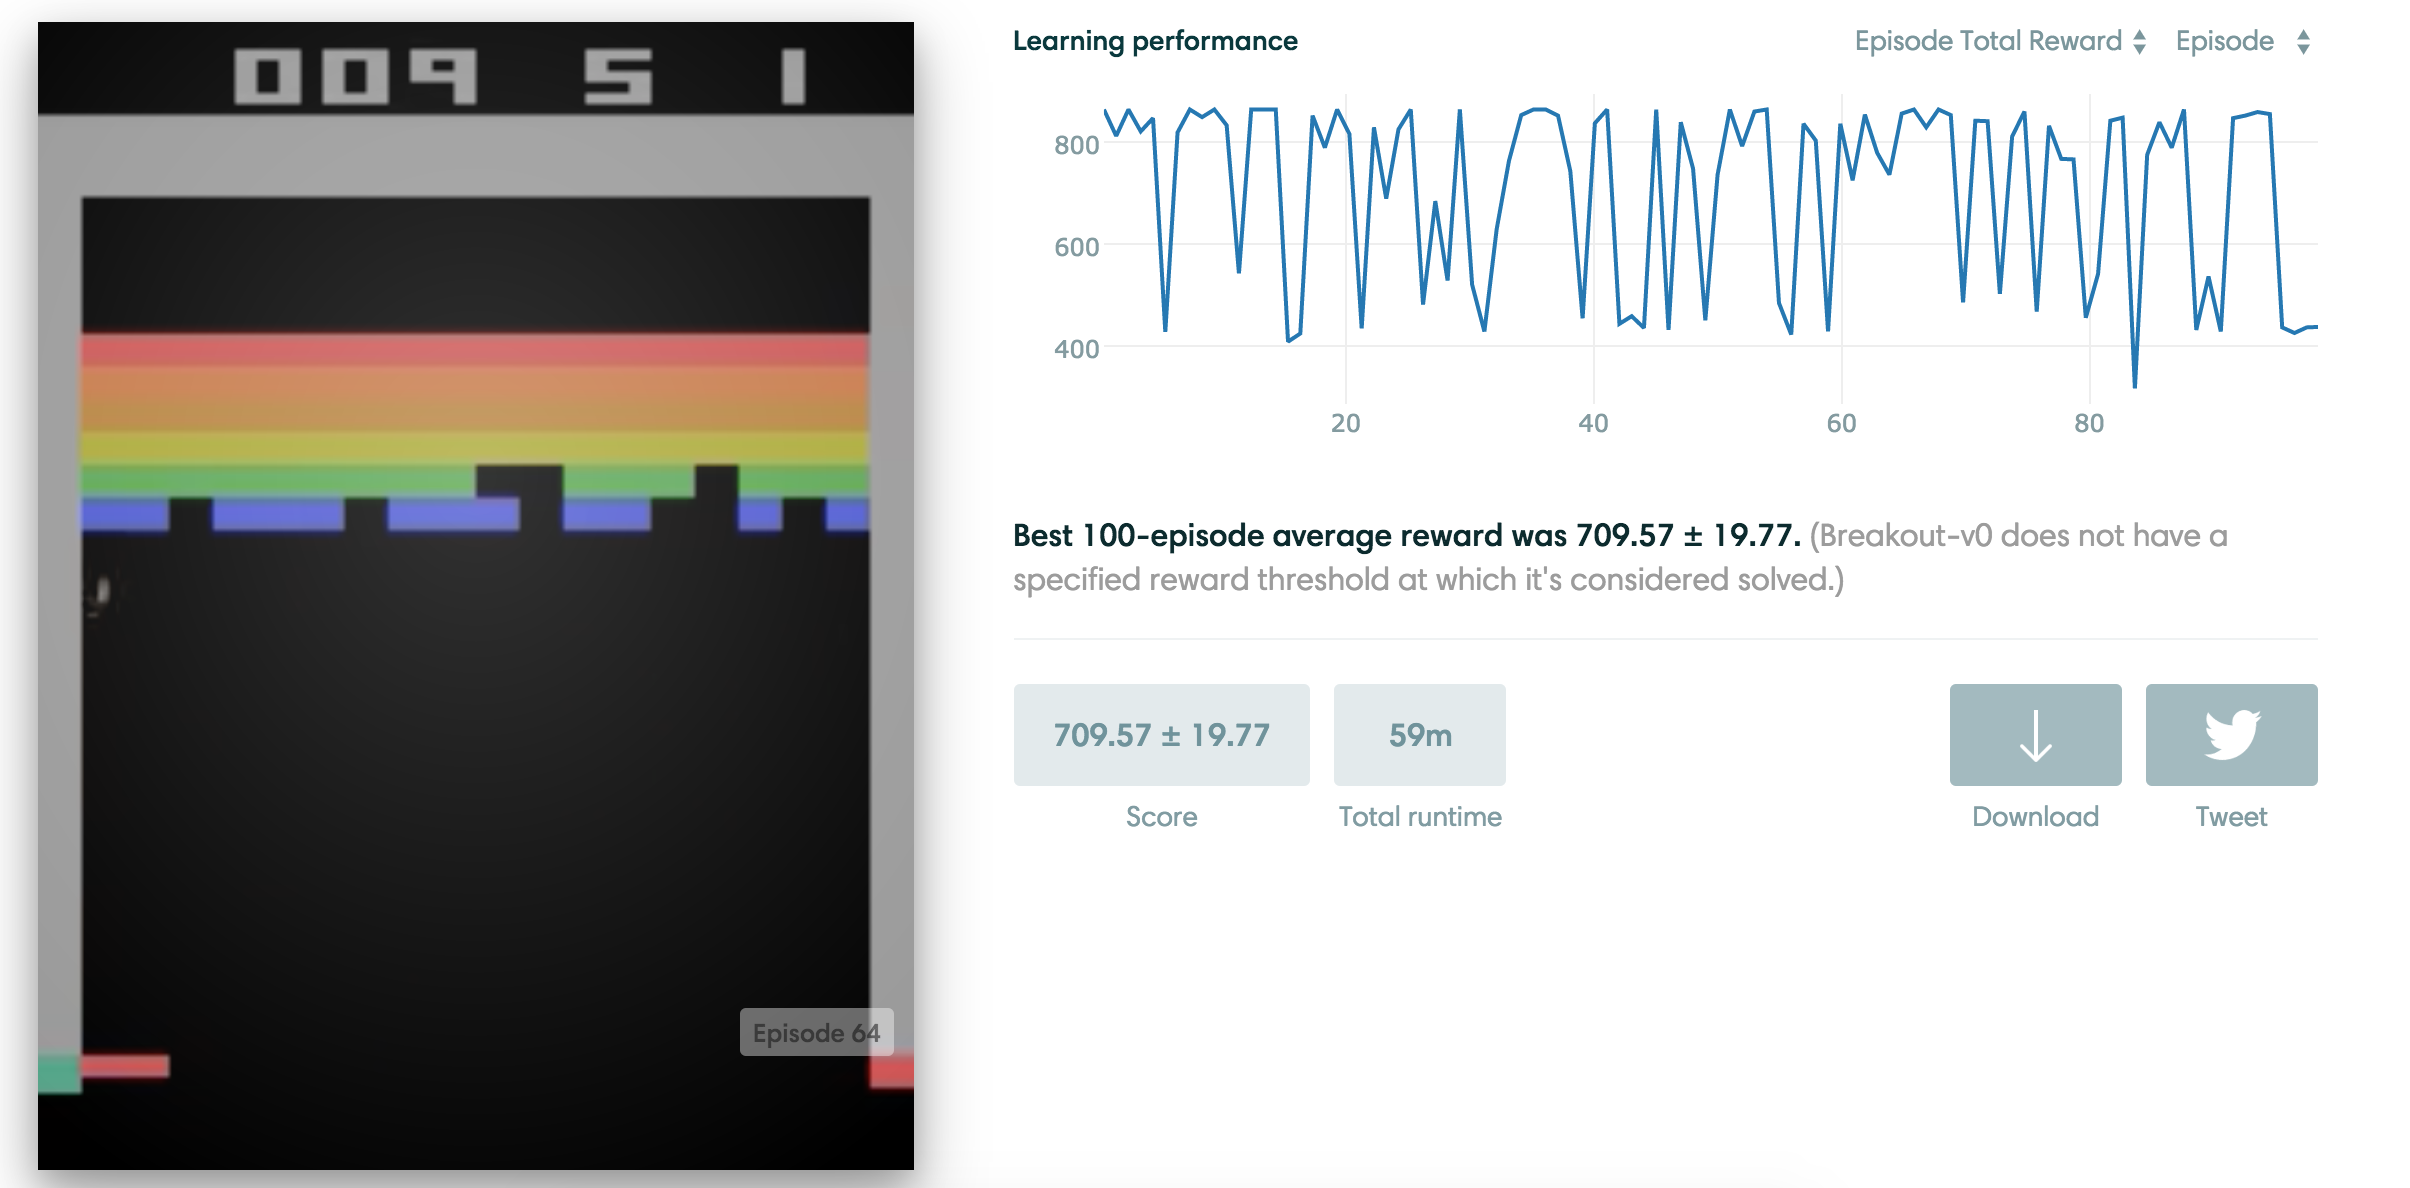
\includegraphics[width=0.49\textwidth]{./fig/A3C_Breakout-v0.png} \\
(a) Breakout-v0 \\
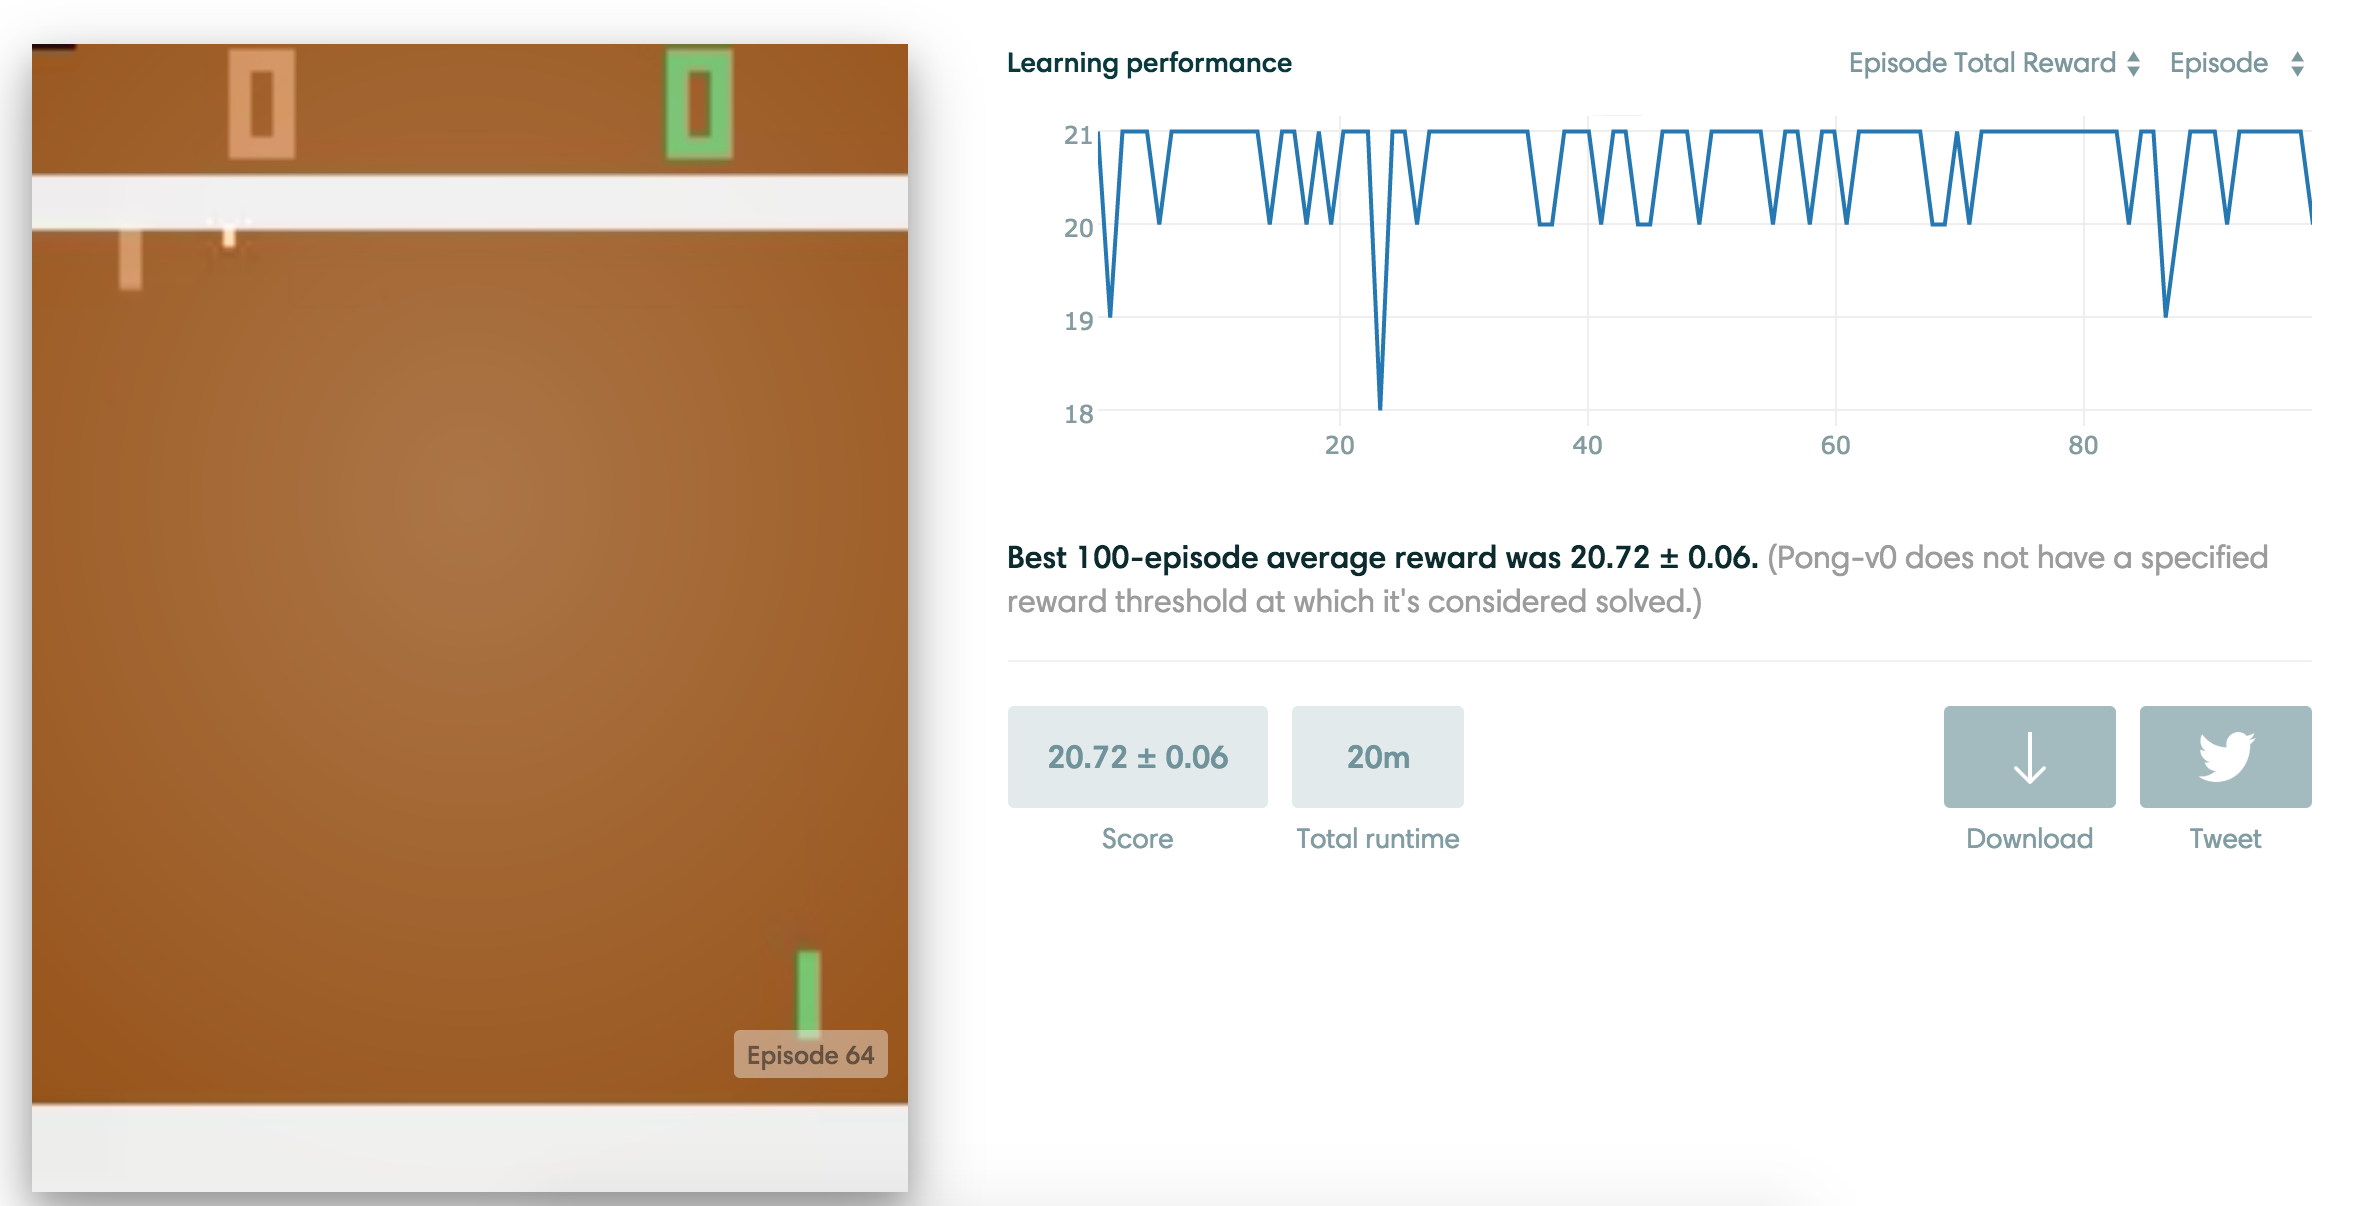
\includegraphics[width=0.49\textwidth]{./fig/A3C_Pong-v0.png} \\
(b) Pong-v0 \\
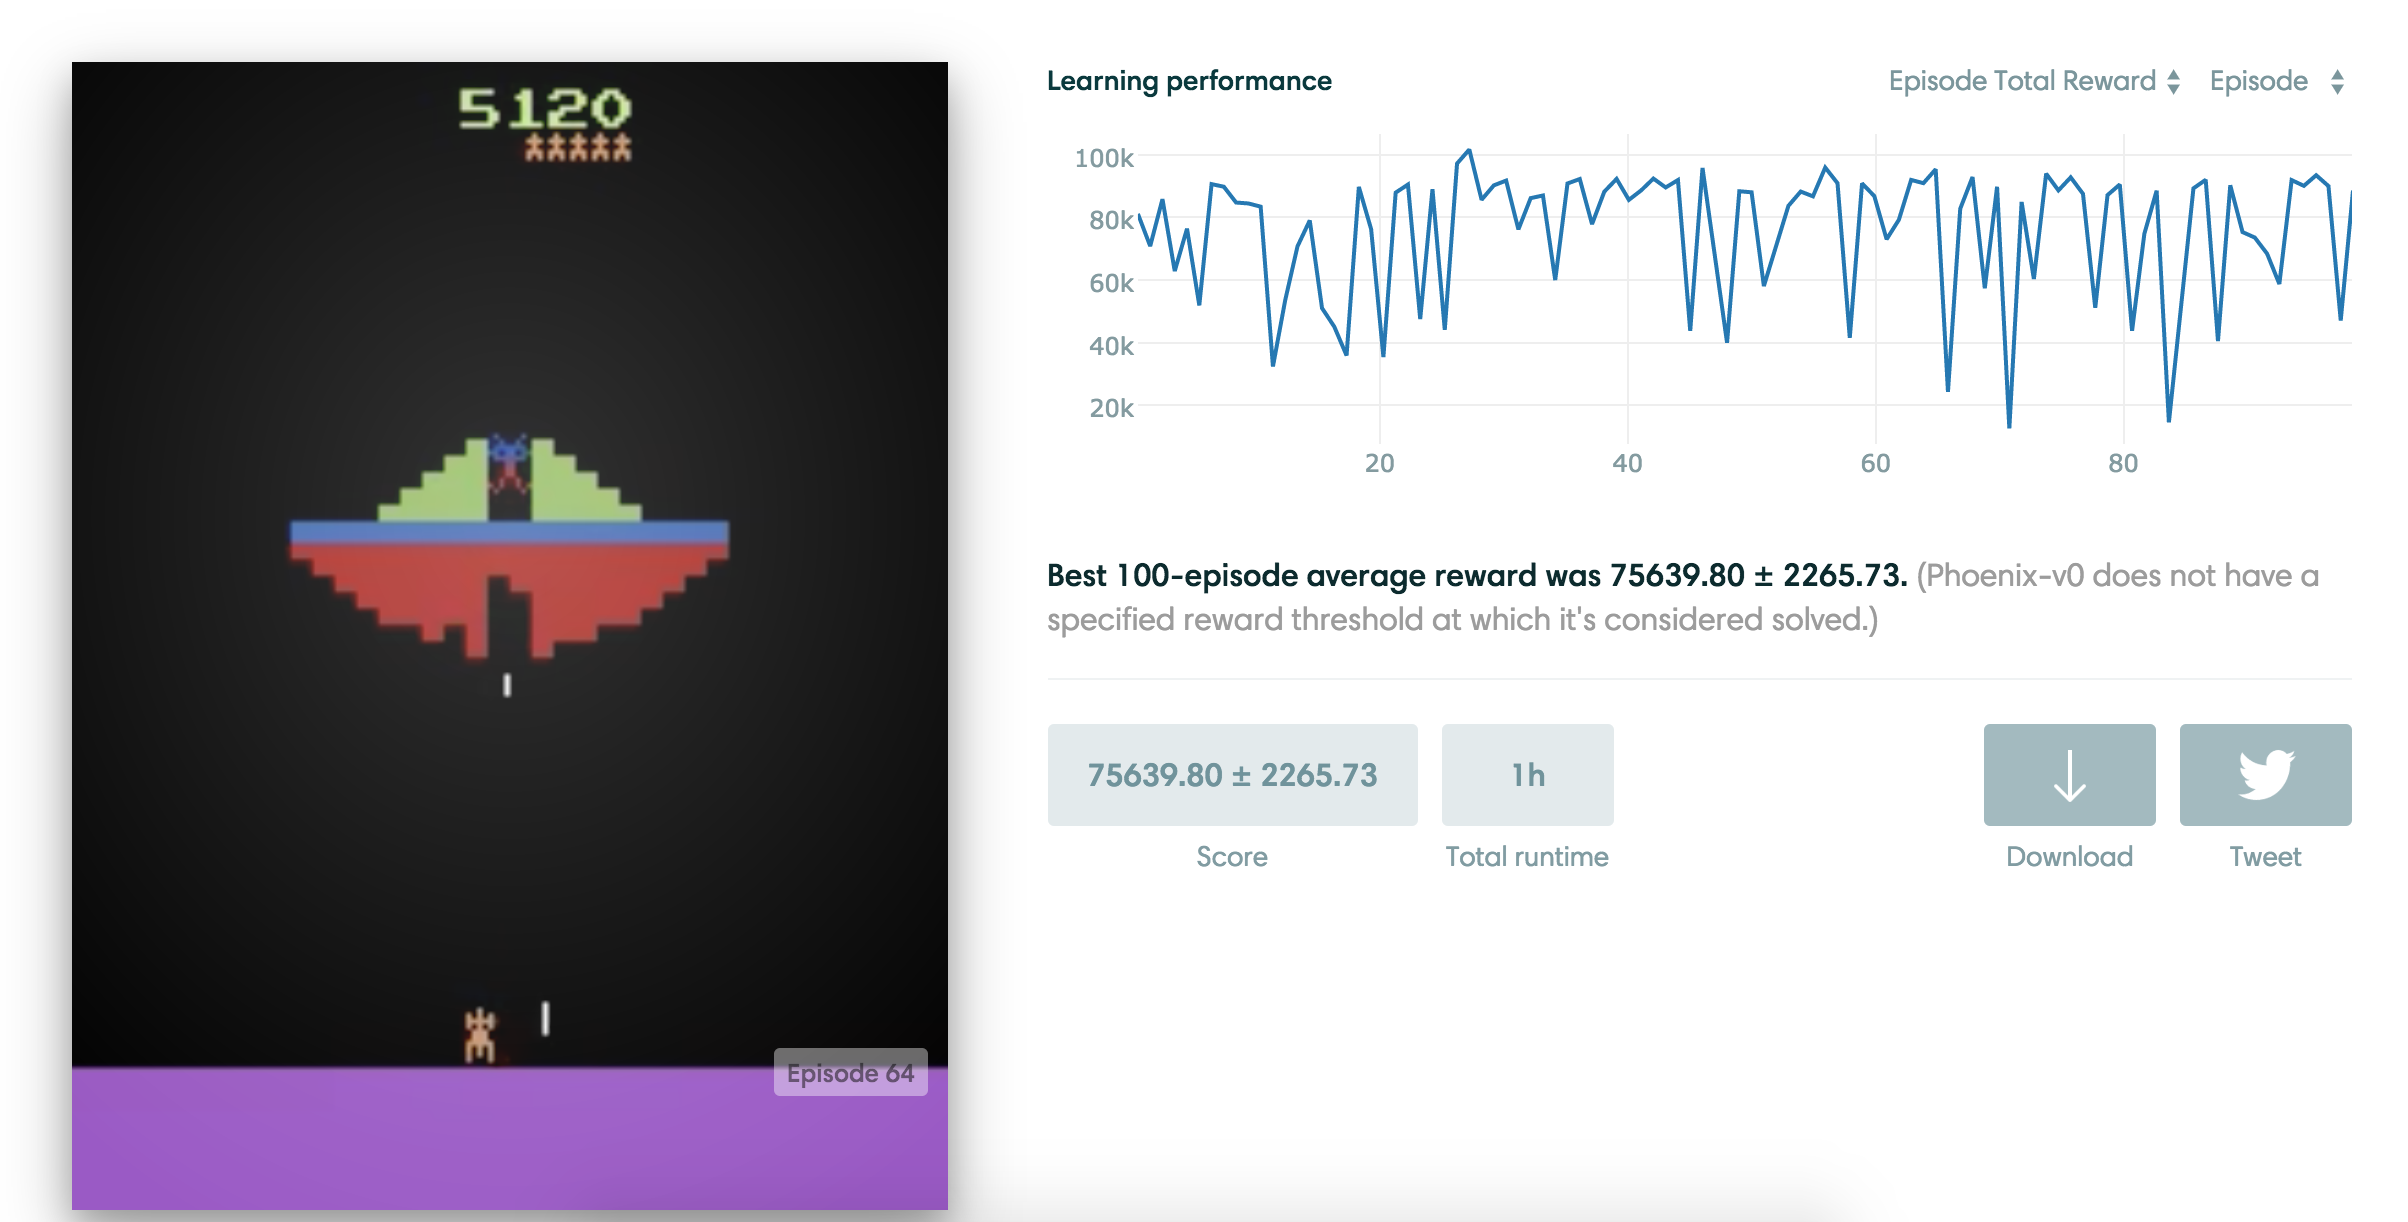
\includegraphics[width=0.49\textwidth]{./fig/A3C_Phoenix-v0.png} \\
(c) Phoenix-v0 \\
\end{tabular}
\label{fig:A3C_baselines}
\caption{The results of 100 epsiodes on three environments by applying A3C algorithms.}
\end{figure}

